\documentclass[10pt,landscape,a4paper]{article}
\usepackage{multicol}
\usepackage{calc}
\usepackage{ifthen}
\usepackage[landscape]{geometry}
\usepackage{hyperref}
\usepackage{graphicx}
\usepackage{tikz}
\usetikzlibrary{positioning,arrows.meta,calc,shapes.callouts,math,decorations.fractals,spy,shapes}
\usepackage{lipsum}
\usepackage{adjustbox}
\usepackage{fancyhdr}

% This sets page margins to .5 inch if using letter paper, and to 1cm
% if using A4 paper. (This probably isn't strictly necessary.)
% If using another size paper, use default 1cm margins.
% \ifthenelse{\lengthtest { \paperwidth = 11in}}
% 	{ \geometry{top=.5in,left=.5in,right=.5in,bottom=.5in} }
% 	{\ifthenelse{ \lengthtest{ \paperwidth = 297mm}}
% 		{\geometry{top=1cm,left=1cm,right=1cm,bottom=1cm} }
% 		{\geometry{top=1cm,left=1cm,right=1cm,bottom=1cm} }
% 	}
\geometry{top=1.5cm,left=1.5cm,right=1.5cm,bottom=1.5cm}

% Turn off header and footer
%\pagestyle{empty}

%\fancyhf{}
\fancyfoot[R]{\today}
\fancyfoot[C]{\thepage}
\pagestyle{fancy}
 

% Redefine section commands to use less space
\makeatletter
\renewcommand{\section}{\@startsection{section}{1}{0mm}%
                                {-1ex plus -.5ex minus -.2ex}%
                                {0.5ex plus .2ex}%x
                                {\normalfont\large\bfseries}}
\renewcommand{\subsection}{\@startsection{subsection}{2}{0mm}%
                                {-1explus -.5ex minus -.2ex}%
                                {0.5ex plus .2ex}%
                                {\normalfont\normalsize\bfseries}}
\renewcommand{\subsubsection}{\@startsection{subsubsection}{3}{0mm}%
                                {-1ex plus -.5ex minus -.2ex}%
                                {1ex plus .2ex}%
                                {\normalfont\small\bfseries}}
\makeatother

% Define BibTeX command
\def\BibTeX{{\rm B\kern-.05em{\sc i\kern-.025em b}\kern-.08em
    T\kern-.1667em\lower.7ex\hbox{E}\kern-.125emX}}

% Don't print section numbers
% \setcounter{secnumdepth}{0}


\setlength{\parindent}{0pt}
\setlength{\parskip}{0pt plus 0.5ex}


% -----------------------------------------------------------------------

\begin{document}

\raggedright
\footnotesize
\begin{multicols}{3}


% multicol parameters
% These lengths are set only within the two main columns
%\setlength{\columnseprule}{0.25pt}
\setlength{\premulticols}{1pt}
\setlength{\postmulticols}{1pt}
\setlength{\multicolsep}{1pt}
\setlength{\columnsep}{2pt}

\begin{center}
     \Large{\textbf{Cheat Sheet}} \\
\end{center}

\section{\LaTeX}
\input{latex/latex.tex}
\newpage
\subsection{adjustbox: adjust boxed content}
\begin{verbatim}
\usepackage{adjustbox}
...
\begin{adjustbox}{
  max totalsize={\textwidth}{\textheight},center}
\end{adjustbox}
\end{verbatim}

\subsection{minipage}
\begin{minipage}[c]{3cm}
  \lipsum[][1-3]
\end{minipage}
\begin{minipage}[c]{3cm}
  \begin{verbatim}
\begin{minipage}[c]{3cm}
  \lipsum[][1-3]
\end{minipage}
  \end{verbatim}
\end{minipage}

\subsection{Beamer class}

\subsubsection{Accessing section names}
\verb |\secname|\\
\verb |\subsecname|\\

\subsubsection{Animations}
Use \verb|%| at the end of the line to avoid interpeting new line causing x-shift in the animation:
\begin{verbatim}
\includegraphics<1>[height=0.5\textheight]{figures/1.pdf}%
\includegraphics<2>[height=0.5\textheight]{figures/2.pdf}
\end{verbatim}
\verb|\visible<3>{...}| Put a set of command visible only on slide 3

\subsubsection{Custom footer}
\begin{verbatim}
\newcommand{\secfoot}{
\begin{tikzpicture}[remember picture, overlay]
  \node [anchor=south,node font=\tiny,text=blue!50]
    (node1) at (current page.south) [] {\secname/\subsecname};
\end{tikzpicture}
}
\end{verbatim}

\subsubsection{Title slide for sections}
\begin{verbatim}
\AtBeginSection[]{
  \begin{frame}
  \vfill
  \centering
  \begin{beamercolorbox}[sep=8pt,center,shadow=true,rounded=true]{title}
    \usebeamerfont{title}\insertsectionhead\par%
  \end{beamercolorbox}
  \vfill
  \end{frame}
}
\end{verbatim}

\subsection{LaTeX default colors -- xcolor package --}
\begin{center}
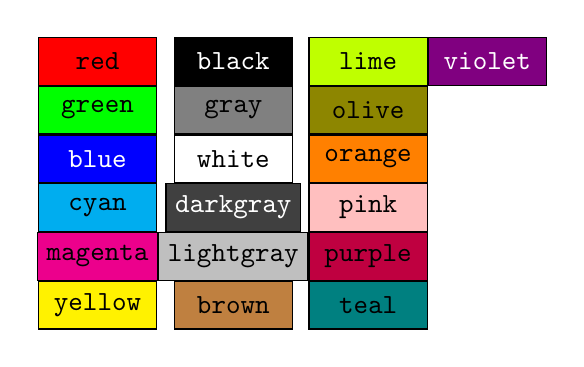
\begin{tikzpicture}[c/.style={minimum width=1.5cm,minimum height=4ex,rectangle,draw}]
  \matrix{
    \node[c,fill=red]{\verb|red|}; &&
    \node[c,fill=black,text=white]{\verb|black|}; &&
    \node[c,fill=lime]{\verb|lime|}; &&
    \node[c,fill=violet,text=white]{\verb|violet|}; \\
    \node[c,fill=green]{\verb|green|}; &&
    \node[c,fill=gray]{\verb|gray|}; &&
    \node[c,fill=olive]{\verb|olive|}; \\
    \node[c,fill=blue,text=white]{\verb|blue|}; &&
    \node[c,fill=white]{\verb|white|}; &&
    \node[c,fill=orange]{\verb|orange|}; \\
    \node[c,fill=cyan]{\verb|cyan|}; &&
    \node[c,fill=darkgray,text=white]{\verb|darkgray|}; &&
    \node[c,fill=pink]{\verb|pink|}; \\
    \node[c,fill=magenta]{\verb|magenta|}; &&
    \node[c,fill=lightgray]{\verb|lightgray|}; &&
    \node[c,fill=purple]{\verb|purple|}; \\
    \node[c,fill=yellow]{\verb|yellow|}; &&
    \node[c,fill=brown]{\verb|brown|}; &&
    \node[c,fill=teal]{\verb|teal|}; \\
  };
\end{tikzpicture}
\end{center}

\subsection{Header and footer}
\begin{verbatim}
\usepackage{fancyhdr}
\fancyhf{}
\fancyfoot[R]{\today}
\fancyfoot[C]{\thepage}
\pagestyle{fancy}
\end{verbatim}

\newpage
\section{\LaTeX\ tikz}
\subsection{General}
\subsubsection{Online TikZ manuel}
\url{https://tikz.dev/}\\
\subsubsection{Package and libraries}
\verb|\usepackage{tikz}| using tikz package\\
\verb|\usetikzlibrary{positioning}| Load a given tikz library\\
\subsubsection{Syntax}
\verb|\coordinate (X) at (3,5);| name a point X\\
\verb|\node[options] (X) at (3,5) {};| place a node and name it X\\

\subsection{Coordinate specifications}
\subsubsection{Coordinate calculations}
\begin{tabular}[]{p{0.1\textwidth}p{0.1\textwidth}l}
&&library needed\\
$(x,y)$&Cartesian coordinates&\\
($\theta$:r)&polar coordinates&\\
\verb |($(A)+{sin(60)}*(B)$)|         &coordinate calculations&calc\\
\verb |($(A)!.25!(B)$)|&                 partway calculations&calc\\
\verb |($(A)!3cm!(B)$)|&                 3~cm from (A) in direction of (B)&calc\\
\verb |($(A)!1.2!30:(B)$)|&              stretch by 1.2, then rotate by 30$^{\circ}$&calc\\
\verb |($(A)!(B)!(C)$)|&                 projection of point B onto line AC&calc\\
\verb |($(A)!(B)!30:(C)$)|&              project B onto line AC, then rotate by 30$^{\circ}$&calc\\
\verb '(n1-|n2)'& projection of n2 on the line passing through n1\\
\verb '(n1|-n2)'& projection of n1 on the line passing through n2\\
\verb |\node[above=1cm of| \verb|somenode.north]|&position new node 1~cm above existing anchor&positioning\\
\end{tabular}
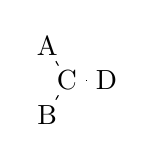
\begin{tikzpicture}
  \node (C) {C}; 
  \node (A) at ($(C)+(120:0.5)$) {A};
  \node (B) at ($(C)+(240:0.5)$) {B};
  \node (D) at ($(C)+(360:0.5)$) {D};
  \draw (C) -- (A);
  \draw (C) -- (B);
  \draw (C) -- (D);
\end{tikzpicture}
\begin{minipage}[c]{3cm}
  \begin{verbatim}
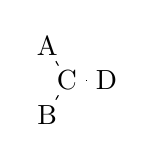
\begin{tikzpicture}
  \node (C) {C}; 
  \node (A) at ($(C)+(120:0.5)$) {A};
  \node (B) at ($(C)+(240:0.5)$) {B};
  \node (D) at ($(C)+(360:0.5)$) {D};
  \draw (C) -- (A);
  \draw (C) -- (B);
  \draw (C) -- (D);
\end{tikzpicture}
  \end{verbatim}
\end{minipage}\\
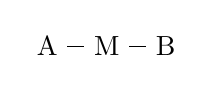
\begin{tikzpicture}
  \node (A) {A};
  \node[right=of A] (B) {B};
  \path (A) -- (B) node[midway] (M) {M};
  \draw (A) -- (M) -- (B);
\end{tikzpicture}
\begin{minipage}[c]{3cm}
  \begin{verbatim}
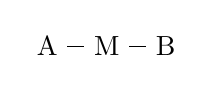
\begin{tikzpicture}
  \node (A) {A};
  \node[right=of A] (B) {B};
  \path (A) -- (B) node[midway] (M) {M};
  \draw (A) -- (M) -- (B);
\end{tikzpicture}
  \end{verbatim}
\end{minipage}\\

\subsubsection{Absolute positioning on the page}
\begin{verbatim}
\begin{tikzpicture}[remember picture, overlay]
  \node [] (node1) at (current page.west) {};
\end{tikzpicture}
\end{verbatim}
\includegraphics[width=0.33\textwidth]{figures/rectangle_shape.pdf}
\subsubsection{Matrix positioning}
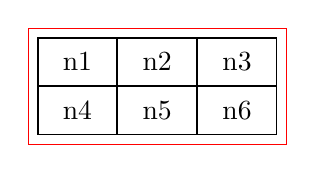
\begin{tikzpicture}
  [n/.style={draw,minimum width=1cm,minimum height=4ex,color=black}]
  \matrix[draw,color=red] (M) {
    \node[n] {n1}; &&
    \node[n] {n2}; &&
    \node[n] {n3}; \\
    \node[n] {n4}; &&
    \node[n] {n5}; &&
    \node[n] {n6}; \\
  };
\end{tikzpicture}
\begin{minipage}[c]{3cm}
  \begin{verbatim}
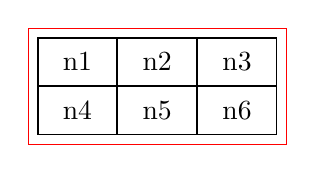
\begin{tikzpicture}
  [n/.style={draw,
             minimum width=1cm,
             minimum height=4ex,
             color=black}]
  \matrix[draw,color=red] (M) {
    \node[n] {n1}; &&
    \node[n] {n2}; &&
    \node[n] {n3}; \\
    \node[n] {n4}; &&
    \node[n] {n5}; &&
    \node[n] {n6}; \\
  };
\end{tikzpicture}
  \end{verbatim}
\end{minipage}

\subsection{Node dimension}
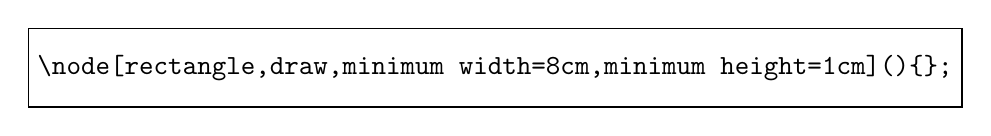
\begin{tikzpicture}
\node[rectangle,draw,minimum width=8cm, minimum height=1cm] () {\verb|\node[rectangle,draw,minimum width=8cm,minimum height=1cm](){};|};
\end{tikzpicture}

\subsection{Node shapes and filling colors}
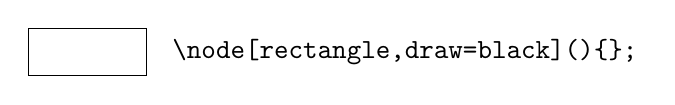
\begin{tikzpicture}
  \node[rectangle,draw=black,minimum width=1.5cm, minimum height=4ex] (rectangle) {}; 
  \node[right=0.2cm of rectangle]{\verb|\node[rectangle,draw=black](){};|};
\end{tikzpicture}
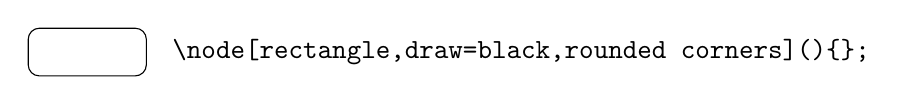
\begin{tikzpicture}
  \node[rectangle,draw=black,minimum width=1.5cm, minimum height=4ex,rounded corners] (rectangle) {}; 
  \node[right=0.2cm of rectangle]{\verb|\node[rectangle,draw=black,rounded corners](){};|};
\end{tikzpicture}

\begin{tikzpicture}
  \node[rectangle,draw=black,minimum width=1.5cm, minimum height=4ex,fill=blue] (rectangle) {}; 
  \node[right=0.2cm of rectangle]{\verb|\node[rectangle,draw=black,fill=blue](){};|};
\end{tikzpicture}

\subsection{Node options}
\subsubsection{Fonts and text colors}
\verb |node font=\tiny|\\
\verb |font=\bfseries| Node font in bold\\
\verb |text=blue| text color\\
\subsubsection{Text alignment in nodes}
\verb 'align=left|center|right' (handling carriage return in nodes)\\
\subsubsection{Style definition}
\verb |\begin{tikzpicture}[stylename/.style={node options...}]| Defining a node style named stylename\\
\verb |node[stylename] (node1) {};| Using a defined style

\subsection{Arrows}
\begin{verbatim}
\coordinate (P1);
\coordinate[right=of P1] (P2);
\end{verbatim}
\begin{tikzpicture}
  \coordinate (P1);
  \coordinate[right=of P1] (P2);
  \draw[->] (P1) -- (P2);
  \node[right of=P2, anchor=west] {\verb|\draw[->] (P1) -- (P2);|};
\end{tikzpicture}
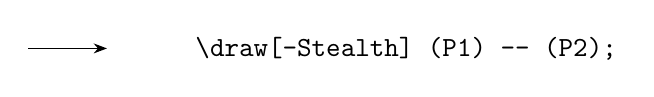
\begin{tikzpicture}
  \coordinate (P1);
  \coordinate[right=of P1] (P2);
  \draw[-Stealth] (P1) -- (P2);
  \node[right of=P2, anchor=west] {\verb|\draw[-Stealth] (P1) -- (P2);|};
\end{tikzpicture}
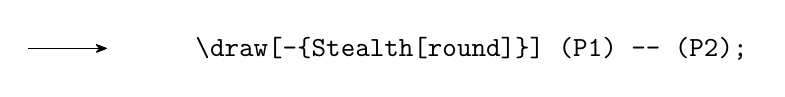
\begin{tikzpicture}
  \coordinate (P1);
  \coordinate[right=of P1] (P2);
  \draw[-{Stealth[round]}] (P1) -- (P2);
  \node[right of=P2, anchor=west] {\verb|\draw[-{Stealth[round]}] (P1) -- (P2);|};
\end{tikzpicture}
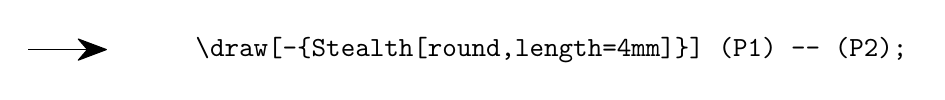
\begin{tikzpicture}
  \coordinate (P1);
  \coordinate[right=of P1] (P2);
  \draw[-{Stealth[round,length=4mm]}] (P1) -- (P2);
  \node[right of=P2, anchor=west] {\verb|\draw[-{Stealth[round,length=4mm]}] (P1) -- (P2);|};
\end{tikzpicture}
\verb |\begin{tikzpicture}[>={Stealth[round]}]| Defining an arrow style for the whole picture\\

\newpage
\section{Makefile}
\subsection{Variables}
\verb|$@|: target name\\
\verb|$^|: first prerequisite\\
\verb|$$X|: Access to the user var. X\\
\subsubsection{Makefile variables}
\begin{verbatim}
foo=World
all:
    echo "Hello ${foo}"
\end{verbatim}

\subsection{Syntax}
\begin{verbatim}
target: prerequisite1 prerequisite2 ...
  commands
\end{verbatim}

\subsection{User defined functions}
\begin{verbatim}
define myfunc
    echo $(1)
    echo $(2)
endef

all:
    $(call myfunc,hello world,hello the universe)
\end{verbatim}

\newpage
\section{Math}
\subsection{Running variance}
$\sigma^{2}=\frac{1}{n(n-1)}\left(n\sum_{i=1}^{n}x_{i}^2-\left(\sum_{i=1}^{n}x_i\right)^2\right)$


\newpage
\section{ImageMagick}
\subsection{Trim an image}
\begin{verbatim}
mogrify -trim <img-file> 
\end{verbatim}
\subsection{Make white color transparent}
\begin{verbatim}
mogrify -transparent white <img-file.png> 
\end{verbatim}


\end{multicols}
\end{document}
